\documentclass{article}
\usepackage{ismir,times,graphicx,url}
\usepackage{txfonts}
\usepackage[utf8]{inputenc}
\usepackage[cyr]{aeguill}
\urlstyle{sf}

%opening
\title{Creating transparent, steerable recommendations}
\author{
Fran\c{c}ois Maillet\\
Sun Microsystems Inc.\\
University of Montreal\\
\texttt{francois.maillet@umontreal.ca}
\and 
Paul Lamere \\
Sun Labs\\
Sun Microsystems Inc.\\
\texttt{paul.lamere@sun.com}
}
\date{September 2008}

\begin{document}

\maketitle

\begin{abstract}

Music recommendation systems are increasingly important in the ever 
    growing world of digital music.  However, most commercial music 
    recommenders rely on collaborative filtering techniques to generate 
    music recommendations. These types of recommendations lack two aspects 
    that are important for recommendation.  First, they lack transparency 
    --- they cannot explain why an item was recommended beyond the trivial 
    ``Other people who listened to X also listened to Y". Second, they 
    lack steerability --- there is no way for a user to interact with the 
    recommender to steer it toward more relevant content.
    
    In this paper we describe the Sun Labs Music Explaura - a 
    web-based application that provides transparent and steerable 
    recommendations. The Music Explaura provides a detailed explanation 
    about why a particular item was recommended and allows a user to 
    steer the recommendations based upon attributes of the music.

\end{abstract}

\section{The Aura}

In our system for recommending items, each musical artist is annotated
by a set of descriptive words and phrases.  The source
of these words can be from text mining the web, from social
annotations, autotagging based upon content analysis, expert
annotation, etc.  One significant source of words in our current
implementation are the social tags from the social music website
Last.fm, mined using the Audioscrobbler web services\footnote{Last.fm's
Audioscrobbler web services described at
http://www.audioscrobbler.net/data/webservices/.}.

Some words such as \textit{rock} and \textit{alternative} are
commonly applied to many artists and therefore are not very descriptive,
while terms such as \textit{shoegaze} and \textit{grindcore} are
less frequently applied (and thus more discriminating).  To emphasize
words that are more descriptive, each term is weighted using the
standard text retrieval weighting function TF-IDF. This
weighting function gives more weight to words that occur more
frequently for a particular item when compared to the frequency of
the word across all items.  The set of weighted tags for an item
is called an item's ``tag cloud'' or in a more poetic way, it's
\textit{aura}.  We use this tag cloud as a representation of
an artist in our system. The similarity between two artists is merely
the cosine similarity between the weighted terms in tag clouds for the artists.



\section{Transparency}
One important key to the success  of a music recommender is to gain the
trust of its users.  One way to gain this trust is to provide
a detailed explanation of why an item was recommended. However,
most commercial music recommenders rely on collaborative filtering
techniques to offer recommendations.  These systems cannot offer
any more detailed explanation of why an item was recommended beyond
the simplistic ``people who liked artist X, also liked artist Y''.
These opaque recommendations do little to garner the  trust of the user.

Since our recommendations are based on the similarity between  the tag clouds
of a preferred item and the recommended item, we can
offer a more detailed explanation of why an item was recommended
by showing how the two tag clouds overlap. Figure \ref{fig:commontags} shows
the overlapping tags for the artists Radiohead and Muse.
Only words common to the two artists are displayed. The size of the
font is determined by the weight of tags and the strength of the
overlap.

\begin{figure}[ht]
\begin{center}
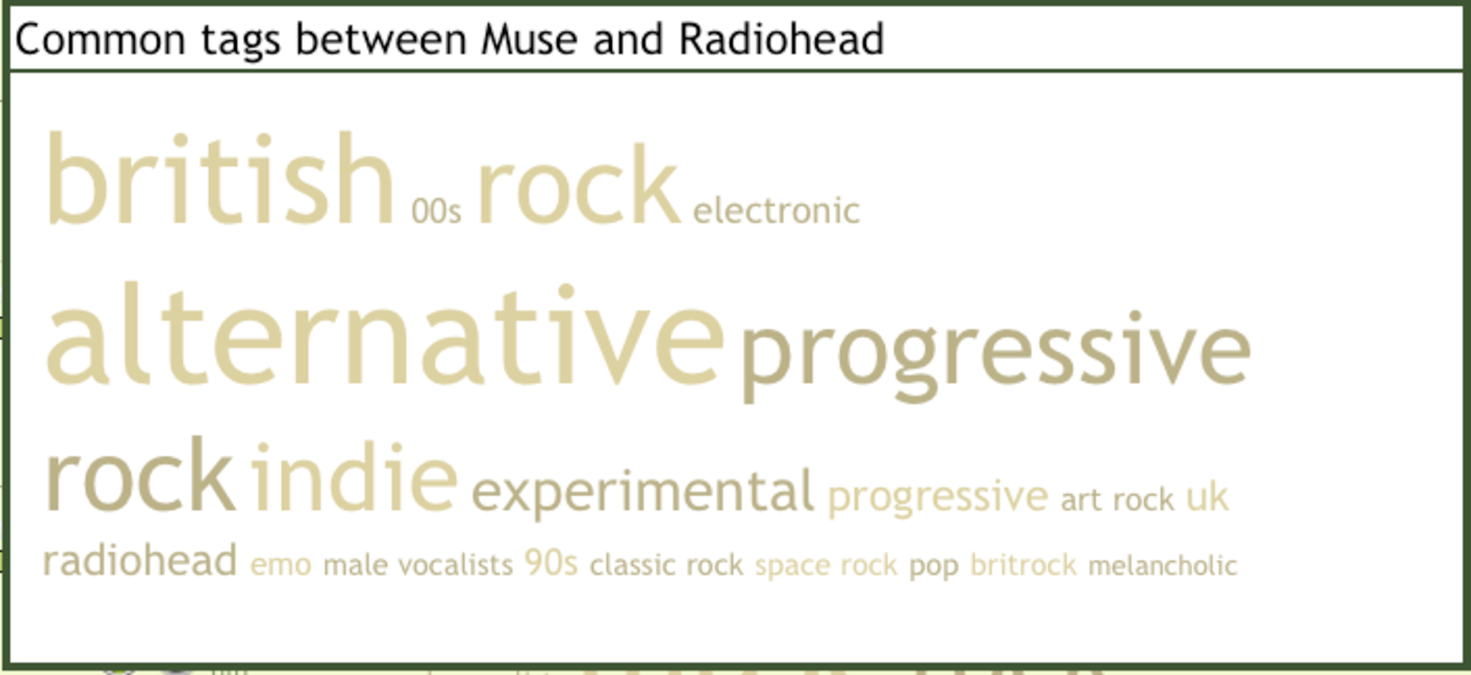
\includegraphics[width=1.0\columnwidth]{radiohead-muse-commontags}
\end{center}
\caption{Common tags between Radiohead and Muse. 
The tags in the 
clouds are weighted by the strength of the overlap between the two clouds.}
\label{fig:commontags}
\end{figure}

\begin{figure*}
\begin{center}
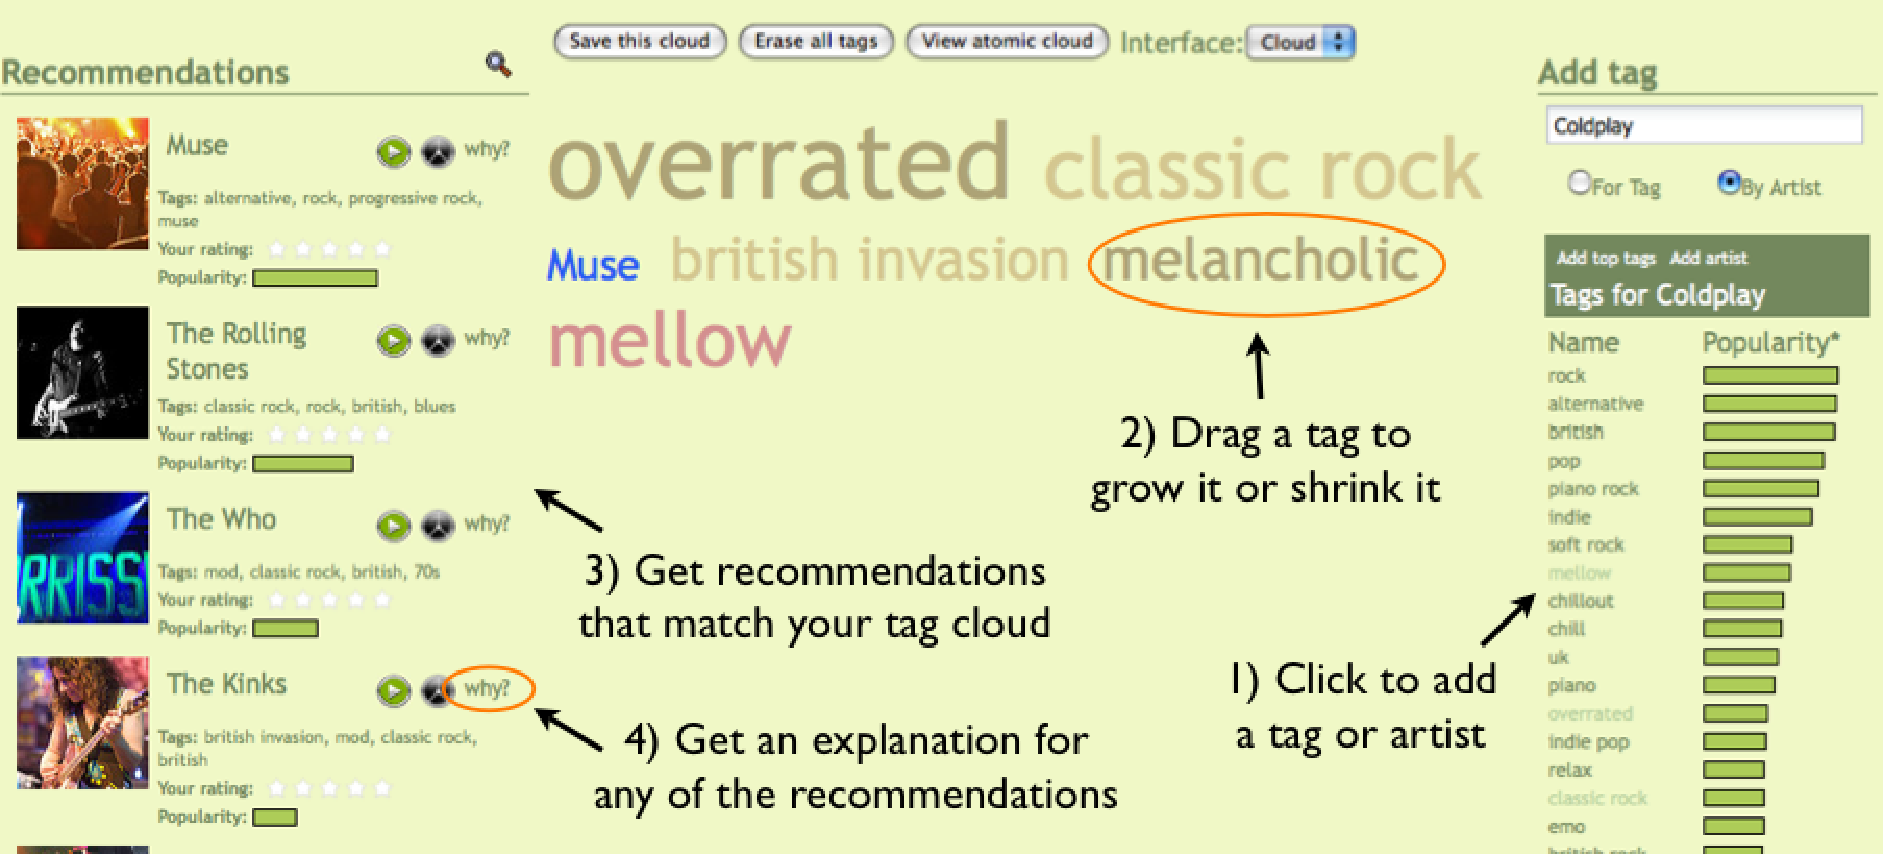
\includegraphics[width=1.00\textwidth]{steerable-withtxt}
\end{center}
\caption{The steerable recommendations interface. Users are able to add tags or artists to the cloud by clicking on them from the right hand panel. Then, they can click and drag them to modify their size. A tag that is shrunk below the size of zero will begin to grow again as a negative tag and act as a filter in the returned recommendations.}
\label{steer}
\end{figure*}

\label{section:steerable}

\section{Steerability}

When a user receives a set of recommendations based upon a seed artist, 
the user may decide that the recommender is giving too much weight to a
certain aspect of the seed artist, and too little weight to another.
In a traditional recommender, there is little that the user can do
guide the recommender toward aspects that the user finds desirable.
With the Music Explaura, a user has much more control over the aspects
that the recommender uses to generate recommendations.  

To steer recommendations with the Music Explaura, a user can interact
with a tag cloud for the seed artist.  The user can add tags, remove
tags or adjust the weight of any tag in the tag cloud.  Whenever
the user makes changes, the set of recommended artists is
immediately updated to include the artists that best match
the new tag cloud.

For example, a fan of 60s psychedelic guitarist Jimi Hendrix could
adjust the Jimi Hendrix tag cloud to give more weight to the
\textit{guitar} tag and less weight to the \textit{60s} and the
\textit{psychedelic} tags to steer the recommender toward guitarists
that sound like Jimi Hendrix, and away from other 60s psychedelia
artists.  The recommender would respond by recommending artists
more like Stevie Ray Vaughan and less like Janis Joplin or The Doors.

Figure \ref{steer} shows an example of the steerable
interface.  In this example, the user has started with a tag cloud based
upon the top tags for the artist Coldplay.  The user has also
added the artist Muse to the cloud. This has the effect
of implicitly including all of the tags for Muse in the tag cloud.  The user can
increase or decrease the weight of an individual tag by
dragging it with the mouse to increase or decrease its size.  The weight of a
tag can even be made negative --- at which point it is colored red.
Tags with negative weights act as filters ---
artists tagged with a negatively weighted tag will not be recommended.  

Whenever the tag cloud is modified, the user
immediately receives an updated list of recommendations.  These are
the artists that most closely match the tag cloud that the user
has constructed. The user can immediately listen to a recommended artist, view
photos of the artist, inspect the tag cloud of an artist or rate the artist.
The user can then update the tag cloud to steer the recommendation 
away from undesirable artists and toward more relevant artists. This
dynamic, iterative approach to recommendation puts the user in control
of the recommender. Contrast this with a traditional collaborative
filtering recommender that typically gives a user no control at all.

\section{Conclusion}
The Music Explaura is a tool for music exploration, discovery and
recommendation that offers transparent, steerable recommendations. With
the Music Explaura, a user can dynamically interact with the
recommender to steer it toward more relevant content and unlike
traditional recommenders, the Music Explaura 
can explain why an item was recommended.
This transparency and interactivity not only helps the user find 
new and interesting music, it also can be more engaging and enjoyable 
for the user.
\end{document}
